\PassOptionsToPackage{square}{natbib}
\documentclass{article}

% if you need to pass options to natbib, use, e.g.:
% \PassOptionsToPackage{numbers, compress}{natbib}
% before loading nips_2016
%
% to avoid loading the natbib package, add option nonatbib:

\usepackage[final]{nips_2016} % produce camera-ready copy

% to compile a camera-ready version, add the [final] option, e.g.:
% \usepackage[final]{nips_2016}

\usepackage[utf8]{inputenc} % allow utf-8 input
\usepackage[T1]{fontenc}    % use 8-bit T1 fonts
\usepackage{hyperref}       % hyperlinks
\usepackage{url}            % simple URL typesetting
\usepackage{booktabs}       % professional-quality tables
\usepackage{amsfonts}       % blackboard math symbols
\usepackage{nicefrac}       % compact symbols for 1/2, etc.
\usepackage{microtype}      % microtypography
\usepackage{graphicx}
\usepackage{color}

\title{Musical Instruments Recognition based on Convolutional Neural Networks}

% The \author macro works with any number of authors. There are two
% commands used to separate the names and addresses of multiple
% authors: \And and \AND.
%
% Using \And between authors leaves it to LaTeX to determine where to
% break the lines. Using \AND forces a line break at that point. So,
% if LaTeX puts 3 of 4 authors names on the first line, and the last
% on the second line, try using \AND instead of \And before the third
% author name.

\author{
  Ci Li\\
  \texttt{cil@kth.se} \\
  %% examples of more authors
  \And
  Mengdi Xue \\
  \texttt{mengdix@kth.se} \\
}

\begin{document}
% \nipsfinalcopy is no longer used

\maketitle

\begin{abstract}
  In this project, we use Convolutional Neural Networks (CNNs) and try different parameter settings to build and train a model for music instruments recognition. We build a base model which consists of two convolutional layers, two max pooling layers, and a fully connected layer. We use the NSynth dataset, which is developed by Google containing high-quality musical notes. We then train the network based on two evaluation methods and finally test the model on real music. As for evaluation, we use accuracy, cross-entropy loss and confusion matrices to measure the performance of our model. 
\end{abstract}

\section{Introduction}

Recently, with the development of digital music creation, there are a large amount of music audio data collected and restored by many organizations. Thus, it is very important to figure out methods to make use of these music data and help people to retrieve the digital audio signal and analyze the content of audio data. Music instrument recognition is one part of these. It is one aspects of audio content analysis, which has a lot of approaches, such as singer recognition, audio information extracting, audio coding, etc. Also, it has a lot of applications, for example, it can be used in content-based music transcription, structured music coding, and music recommending and query engines, etc. So in this project we want to recognize different music instruments due to the above reasons. In previous research on music instrument recognition, models like logistic regression, K-NN, SVM \cite{sell}, Naive Bayes model, multilayer perceptron (MLP), Radial Basis Functions (RBFs) \cite{deng}, quadratic discriminant analysis \cite{agostini}, etc. are applied. As for feature extracting, Mel-frequency cepstral coefficients (MFCC) features, linear prediction cepstral and delta cepstral coefficients are commonly used in musical instrument recognition . But MFCC performs better in music instrument recognition according to \cite{eronen}. In our project, we tried another model based on MFCC feature.

Deep Neural Networks (DNNs) is one of the machine learning tools based on multi-layer feed-forward artificial neural networks. It is designed to imitate human brain structure and is used to recognize patterns. Convolutional Neural Networks (CNNs) is one variant of DNNs, which is also a kind of feed-forward artificial neural networks. They are now successfully applied to many scientific fields and become a new trend because CNNs avoid the complex pre-processing of the image, and people can use the original image as the input directly. CNNs are also known as shift invariant or space invariant artificial neural networks (SIANN), based on their shared-weights architecture and translation invariance characteristics.\cite{zhang} As a result, people use CNNs to convolute the image, audio or video image and try to recognize features based on convolutional parts of the images. They have outstanding performances in image and video recognition \cite{krizhevsky} and successful applications in music recommending systems \cite{vanden} and automatic speech recognition (ASR) systems \cite{abdelhamid}. CNNs have also been successfully applied to musical instrument recognition in real-world polyphonic music \cite{yoonchang}. But it also has limits that it needs a large amount of computational resources to run, which has not yet been solved.

Since CNNs has been successfully applied to image recognition systems, ASR systems and even musical instruments recognition systems, in our project, we applied CNNs architecture on MFCC feature of the audio data of different instruments with variant notes and tried to classify their music instruments family. The goal of our project is to build models to recognize music instrument with CNNs, try different parameter settings to see their performances and apply the model on real data. We will use the same CNNs architecture to train our model and evaluate how they perform based on their accuracy, loss and confusion matrices. In Section 2, we describes our CNNs architecture and data representation. Next, we show details of our experiments in Section 3 and the performances of the experiments in Section 4. Finally, Section 5 contains our discussions and conclusions based on our experiments.

% 最后介绍一下其他的section

\section{Method}

\subsection{Model Architecture}

As mentioned earlier, CNNs are successfully applied to ASR and image recognition fields. That is because, in the image and speech domain, using traditional neural networks will consume too much computational resources. Usually, the size of MFCC feature of an utterance is a two-dimension matrix that has length of the time length (assume it's \emph{t} here) and width of \emph{13} according to MFCC feature extraction. If a traditional fully connected network structure is used, which means the nerves in the network will be connected to each neuron on the adjacent layer, then each  layer of the network will have \emph{13*t} neurons (t=299 here). Assume we have \emph{m} hidden nodes and have output size of \emph{n}, then the size of weight parameter we need will be \emph{13*t*m*n}, which will be too large if we have long time sequences and too much classes to recognize. However, CNNs will solve this problem.

In this project, we applied a typical CNNs architecture on our MFCC features. It is composed of two convolutional layers, two max pooling layers, one fully connected layer with softmax, as in Figure \ref{fig:cnn}. We will introduce them in detail in the following.

\begin{figure}[h!]
\centering
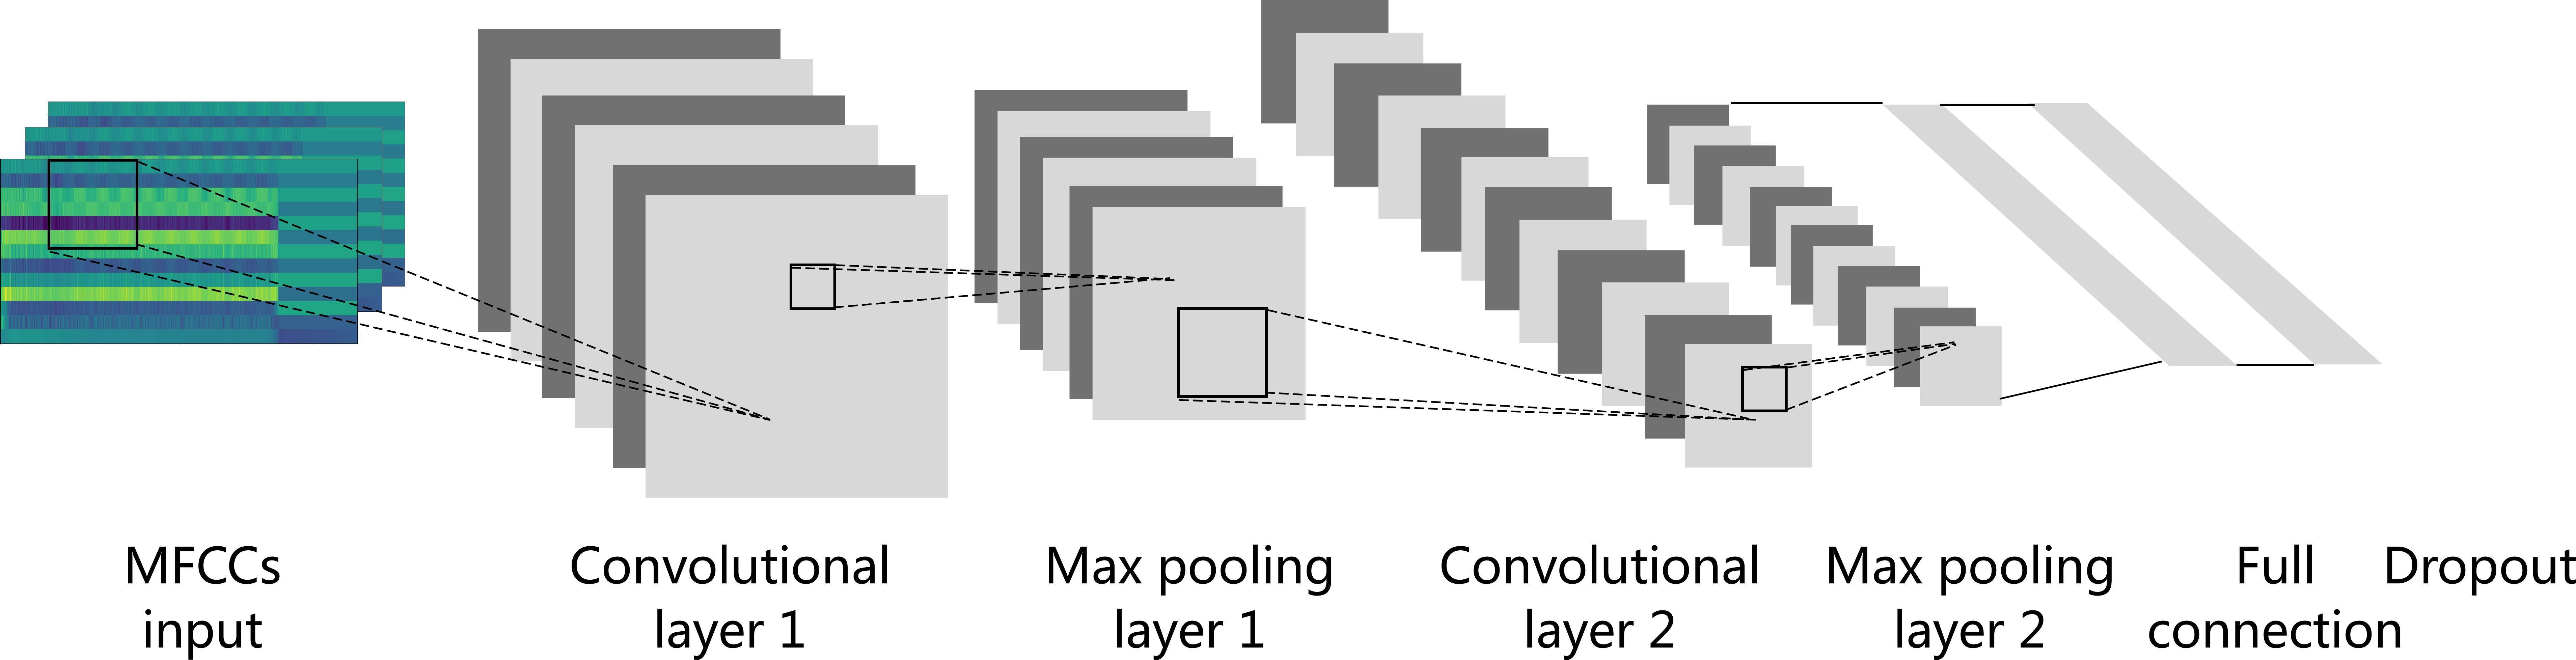
\includegraphics[width=\textwidth]{cnnarchitecture.png}
\caption{CNNs architecture overview}
\label{fig:cnn}
\end{figure}

Firstly, the convolutional layer is accomplished by applying a number of filters, which is also called kernels, to the input matrix. It convolves the input matrix with each filter, slides the filter over all spatial locations in image and outputs one number each time, which is the dot product between the filter and the convolved input matrix that has the same size of the filter. Then, the features are correlated in each output and the outputs will be stacked together. This means the convolutional kernels can extract, or detect specific features of the original input and stacking all they learned together to get a global result. Usually, we use the first convolutional layer to find basic features and apply the second convolutional layer to find some relatively complex features based on the basic features. Bigger size of convolutional kernels will embody more detailed features of the input. In our architecture, the two convolutional layers both have filter size of 5 by 5. The first layer has 32 filters and the second layer has 64 filters.

Then, after each convolutional layer, a pooling layer is applied to each window to return a more independent value of each filter as the output. The commonly used pooling methods are finding the maximum value, average, or median value. The goal of pooling is to extract the independent features that are more representative so that after subsequent calculations, the size of the feature map, the size of parameters, and the amount of calculation are reduced, but the effect is not lost. In our architecture, we applied max pooling as usual to extract the largest value of the window to represent each window. So, using this CNNs network, the size of the weight parameter we need is \emph{5*5*32} in the first convolutional layer and \emph{5*5*64} in the second convolutional layer. The original input here is \emph{299*13}. After the convolutional part, the output is \emph{73*2}. So the parameters for fully connected layer is \emph{73*2*m*n}. We can see that the amount of parameters we need here is much less than only using fully connected network, which needs \emph{13*299*m*n}.

After the second max pooling layer, usually, a fully connected layer with softmax will be used to classify. The output of the second max pooling layer will be flattened to vectors and used as input of the fully connected layer. In our architecture, we applied one fully connected layer with 1023 hidden nodes and a softmax output. And we added a dropout layer with value of 0.8 to improve the generalization of the network \cite{srivastava}.

To evaluate the network, a cross entropy loss was applied to calculate the loss of training set and validation set. In neural networks, cross entropy function is usually used with softmax classifier. Softmax classifier calculates the probability vector the network assigns to the input for each class, and cross entropy loss computes the negative log-likelihood of the training data, as in Equation \ref{con:crossentropy}.

\begin{equation}
L(D, W, b)=-\frac{1}{|D|}\sum_{(x,y)\in D}log(\frac{exp(s_y)}{\sum_{k=1}^{C} exp(s_k)}) \label{con:crossentropy}  
\end{equation}

As for the gradient optimization, Adam optimizer is applied in our architecture. It is a method for efficient stochastic optimization that only requires first-order gradients with little memory requirement.\cite{adam} It is based on stochastic gradient descent, which is more efficient, more suitable for solving optimization problems with large scale data and parameters, more suitable for solving problems with high noise or sparse gradients, and needs less adjustments of parameters.

\subsection{Data Representation}

\subsubsection{The NSynth Dataset}

The NSynth\cite{nsynth} is an audio database released by Google containing high-quality musical notes. The NSynth has 1006 standard instruments with totally 11 instrument families including Bass, Brass, Flute, Guitar, Keyboard, Mallet, Organ, Reed, String, Synth Lead, and Vocal. Each family includes different audio samples with different velocities ranging over different pitch of a standard MIDI piano. Each audio file contains four seconds audio of the corresponding instrument with multiple features in note. The NSynth provides data in two formats: one is tfrecord, which can be directly used in Tensorflow, and another is raw audios in format of wav files. There are totally 289,205 samples in training set, 12,678 samples in validation set and 4,096 samples in testing set. 

\subsubsection{Feature Extraction}

Mel-frequency cepstral coefficients (MFCCs) are coefficients that collectively make up an Mel-frequency cepstral (MFC) which is a representation of the short-term power spectrum of a sound.\cite{mfcc} MFCCs is one of the audio features usually used in Speech Technology and music genre classification. 

\begin{figure}[h!]
\centering
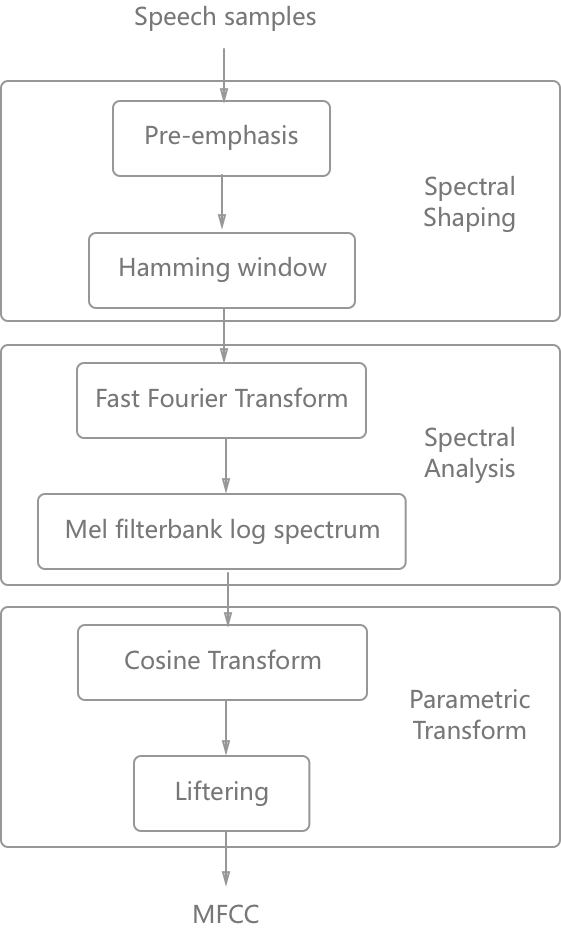
\includegraphics[width=0.3\textwidth]{mfcc-process.png}
\caption{MFCC process}
\label{fig:mfcc}
\end{figure}

MFCCs is generated by 6 steps shown in Figure \ref{fig:mfcc}. Firstly, it enframes the input to extract frames of samples over time from the input speech sample taking the value of frame length in samples and the shift of consecutive windows in samples into account. Next, the pre-emphasis step is a high frequency filter to emphasize the energy of high frequency which is suppressed by the pronunciation system in each frame. Next step of spectral shaping is to apply hamming window to the frames of speech signal in order to smooth the values and reduce spectral leakage. Then, it comes to spectral analysis part. Fast Fourier transform(FFT) converts the signal in time domain to energy distribution in the frequency domain. Different energy distribution can represent different characteristics of different voice. However, human ear is sensitive to different frequency bands. So the Mel filterbank log spectrum can help the signal fit the property of non-linear human ear perception of sound. The last part is parametric transform. After discrete cosine transform(DCT), the energy will focus on the media and the low frequency part, so it is common to use the top 13 coefficients as the result of DCT. Finally liftering function is used to correct the range of the coefficients.


% 来一段mfcc的介绍科科。\\ 
% 哇通过分段,预加重,加窗,傅立叶变换,三角滤波,DCT。经过DCT之后,中低频的数据包含大部分信息,所以只取了前13维作为数据,再过一个lifter,生成极具特色的mfcc。\\

\section{Experiments}

In this section, we will present our result of the experiments using tensorflow to build CNNs on the MFCCs features of the NSynth dataset. We will also provide results of some variations of the model in section 2 to try to analyze the influences of different parameters.

\subsection{Data Pre-processing}

The overall data processing is as following. We read the sampling rate, musical instrument family and audio data from the tfrecord file of each dataset. Then we calculated the lifted MFCCs of each utterance using their audio data and sampling rate and stored them with their target instrument family. So we have 289,205 samples in training set, 12,678 samples in validation set, and 4,096 samples in testing set.

Secondly, all the samples in the dataset contains 4 seconds of records with 1 second silence in the end. At first, we used the whole sample for experiment including the last second of silence, but we found that the network gave random predictions sometimes. We think it is because the training data has too much low frequency component, which is the silence part. So we decided to use the first 3 seconds of each sample for experiment to have more accurate results.

The training dataset has 289,205 samples in total but the data for each classes are unbalanced as shown in Table \ref{tab:dataset}. It is known that machine learning classifiers may fail to deal with imbalanced training datasets because they are sensitive to portions of different classes. So we pre-processed the training set in order to have balanced data for training. In order to achieve this, we randomly sampled 10,000 utterances with replacement from each class for training and shuffled the examples for the network to convergence faster. Eventually, we have 110,000 training data in total. Also, we normalised over the whole training set, calculated the means and covariances and stored them to normalise the validation set and testing set when using them.

\begin{table}[h]
  \caption{NSynth: size of each class in every dataset}
  \label{tab:dataset}
  \centering
  \begin{tabular}{llllllllllll}
    \toprule
    Dataset  &Bass	& Brass	& Flute	& Guitar	& Keyboard	& Mallet\\
    \midrule
    train & 62836	& 11789	& 8303	& 30609	& 49417	& 33538\\
    test & 2638	& 886	& 470	& 2081	& 2404	& 663\\
    valid & 3481	& 1155	& 650	& 2733	& 3170	& 865\\
    total & 68955	& 13830	& 9423	& 35423	& 54991	& 35066\\
    \toprule
    Dataset  & Organ & Reed	& String    & Synth	& Vocal\\
    \midrule
    train	& 32879	& 13191	& 18660	& 5501	& 9804\\
    test   & 1598	& 720	& 814	& 0	    & 404\\
    valid    & 2100	& 955	& 1120	& 0	    & 545\\
    total   & 36577	& 14866	& 20594	& 5501	& 10753\\
    \bottomrule
  \end{tabular}
\end{table}

\subsection{Experimental Setup}

In our experiments, we used Tensorflow to build our CNNs architecture for training. Tensorflow is a deep learning framework provided by Google, which supports multiple platforms. It can run both on CPUs and GPUs and provides rich libaries for different algorithms, architectures and frameworks. As a result, we used it to build CNNs and run our model on GPUs. CNNs need a lot of computations based on matrices and convolutions, so GPUs can help CNNs to compute much faster than CPUs.

% 我觉得可以在架构图上写上我们的size
Our MFCCs record has size of 299 by 13. The basic settings we used is the typical 32 kernels for the first convolutional layer and 64 kernels for the second convolutional layer, which are all of size 5 by 5. And we used two max pooling layer of size 2 by 2 after each convolutional layer. So the output of our convolutional part is 73 by 2. Then we used mini-batch training with Adam algorithms to train. As for evaluating, we calculated the cross entropy loss for both training set and validation set. We only sampled 200 samples from validation set each time to save calculation time because the validation set is too large here. Eventually, we calculated and output the final accuracy and loss of the training set, the validation set and the testing set.

\subsection{Experimental Parameters}

Since we used CNNs in our experiments, the main parameters for setting is the filter size, batch size, step size, learning rate, and number of epoches.

In the following section, we will present the results based on different batch sizes. However, for other parameters, we have the following settings as default settings:

\setlength{\parindent}{5ex}
$learning\_rate = 1e-4$\par
\setlength{\parindent}{5ex}
$training\_epochs = 70$\par
\setlength{\parindent}{5ex}
$steps = train\_data\_size/batch\_size$\par

\section{Results}

% \subsection{Base Result}

% Our basic architecture has the same parpameters as described in 3.3. Then we computed their loss trends and accuracy trends of the training set and the validation set during training. The shadow orange line is the original loss calculated based on each training batch and the orange line is the smoothed trend of the training loss. Similarly, the shadow blue line is the original loss calculated on 400 sampled validation data and the blue line is the smoothed trend of the validation loss. The result is as in Figure \ref{fig:accuracy_loss_400}. It can be seen that the trend of the validation loss is decreasing so the model does not overfit. The result accuracy of the whole training set is 92.89\%, accuracy of the whole validation set is 34.44\% and the accuracy on testing set is 34.02\%.

% \begin{figure}[h!]
% \centering
% 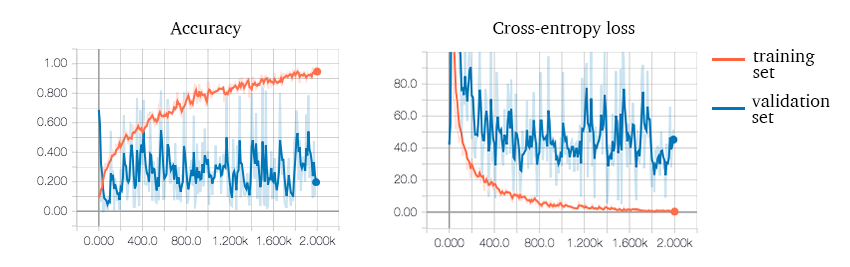
\includegraphics[width=\textwidth]{accuracy_loss_400.png}
% \caption{Accuracy and loss of the training set and the validation set}
% \label{fig:accuracy_loss_400}
% \end{figure}

% \subsection{Results of different batch size}

% Then we changed the batch size smaller to 200 and use the same settings for other parameters. The result accuracy and loss is as in Figure \ref{fig:accuracy_loss_200}. The result accuracy of this model on training set is 97.07\%, on validation set is 37.37\% and on testing set is 37.20\%. We can see that the behavior of this model is better than the model using batch size of 400. Also, the trend of the loss of training and validation on this model decreases much faster than the previous model.

% \begin{figure}[h!]
% \centering
% 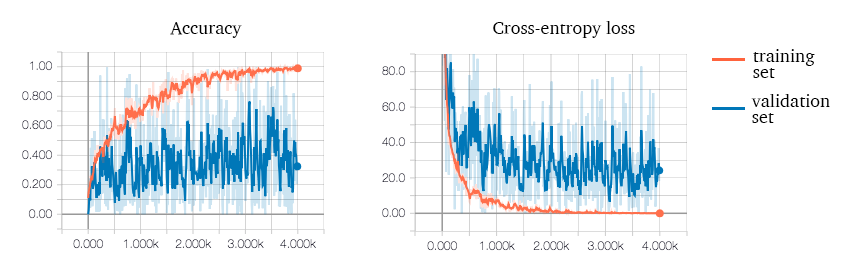
\includegraphics[width=\textwidth]{accuracy_loss_200.png}
% \caption{Accuracy and loss of the training set and the validation set}
% \label{fig:accuracy_loss_200}
% \end{figure}

% \subsection{Results of training with three subsets}

% When we extracted the dataset, we separated them into 3 subsets for easier storing. So we tried to fit the model on the subsets one by one and store the model when the training of each subset is done for the next subset to train. Here we use batch size of 200. The accuracy and loss of this model is as in Figure \ref{fig:accuracy_loss_200_apart}. We can see that the accuracy and loss have a stepped form. Every time when we use the old model and a new subset to train, the accuracy on the training set goes down a little and correspondingly, the loss increases a little. But the overall trend of validation set is better than the above 2 models.

% \noindent Based on this model, we get accuracy on training set of 97.23\%, on validation set of 45.81\% and on testing set of 44.87\%. The accuracy after each subsets is as in Table \ref{tab:accuracy_loss_200_apart}.

% \begin{figure}[h!]
% \centering
% 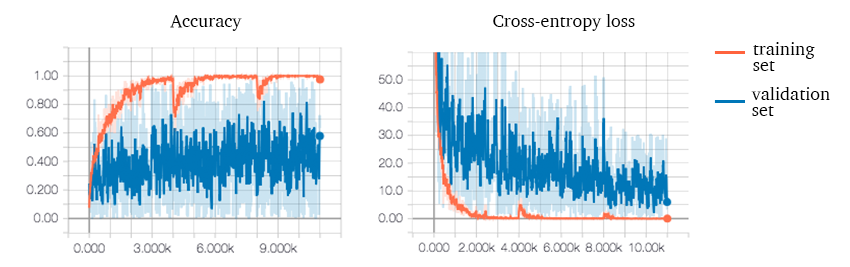
\includegraphics[width=\textwidth]{accuracy_loss_200_apart.png}
% \caption{Accuracy and loss of the training set and the validation set}
% \label{fig:accuracy_loss_200_apart}
% \end{figure}

% \begin{table}[t]
%   \caption{Accuracy after training of each subsets}
%   \label{tab:accuracy_loss_200_apart}
%   \centering
%   \begin{tabular}{llll}
%     \toprule
%     Subset  &Training	& Validation	& Test\\
%     \midrule
%     1 & 95.89\%	& 38.09\%	& 38.05\%\\
%     2 & 97.91\%	& 42.54\%	& 41.80\%\\
%     3 & 97.23\%	& 45.81\%	& 44.87\%\\
%     \bottomrule
%   \end{tabular}
% \end{table}


\subsection{Base Result}

Our basic architecture has the same parameters as described in 3.3. Then we computed their loss trends and accuracy trends of the training set and the validation set during training.

\noindent In our experiment, the accuracy is computed based on the top probability and top two probabilities among the predictions. We calculated the accuracy based on the top two probabilities because there are 11 classes in total so that a certain extent of errors are allowed. The result based on the top probability is as in Figure \ref{fig:accuracy_top1} and the result based on the top two probabilities is shown in Figure \ref{fig:accuracy_top2}. The shadow orange line is the original loss calculated based on each training batch and the orange line is the smoothed trend of the training loss. Similarly, the shadow blue line is the original loss calculated on 200 sampled validation data and the blue line is the smoothed trend of the validation loss. It can be seen that the trends of accuracy and loss are the same within two evaluation methods. The validation loss is decreasing along the time, which means that the model does not overfit. The result accuracy of the these two different evaluation methods are shown in Table \ref{tab:accuracy_2_evaluation}.

\begin{table}[h]
  \caption{Accuracy based on two evaluation methods and different batch sizes}
  \label{tab:accuracy_2_evaluation}
  \centering
  \begin{tabular}{llll}
    \toprule
    Methods  &Training	& Validation	& Test\\
    \midrule
    Batch size 200, Top one probability & 94.57\%	& 41.40\%	& 42.45\%\\
    Batch size 200, Top two probabilities & 97.75\%	& 59.88\%	& 60.175\%\\
    Batch size 400, Top one probability & 97.07\%  & 37.37\%  &  37.20\%\\
    \bottomrule
  \end{tabular}
\end{table}

\begin{figure}[h!]
\centering
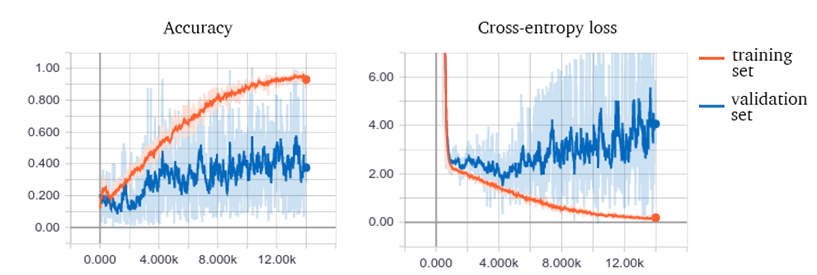
\includegraphics[width=\textwidth]{accuracy_top1.png}
\caption{Accuracy and loss curve of results based on top probability on validation and testing sets}
\label{fig:accuracy_top1}
\end{figure}

\begin{figure}[h!]
\centering
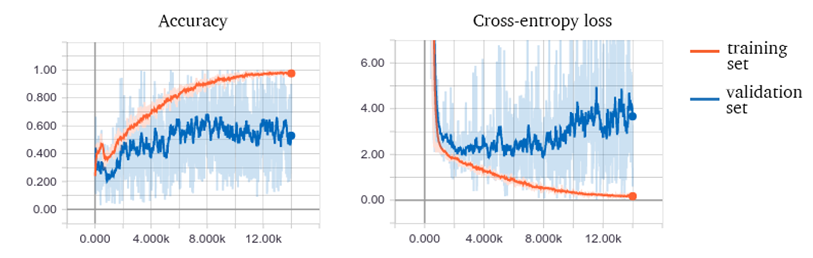
\includegraphics[width=\textwidth]{accuracy_top2.png}
\caption{Accuracy and loss curve of results based on top two probabilities on validation and testing sets}
\label{fig:accuracy_top2}
\end{figure}

\begin{figure}[h!]
\centering
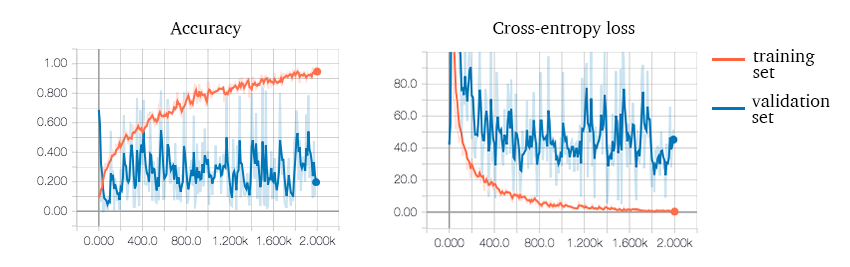
\includegraphics[width=\textwidth]{accuracy_loss_400.png}
\caption{Accuracy and loss curve of results based on top probability on validation and testing sets with batch size 400}
\label{fig:accuracy_top1_400}
\end{figure}

\noindent From the accuracy table we can see the test accuracy based on top two probabilities is 60.175\% while the accuracy based on top one probability is 42.45\%. This means that the probabilities of the right answers appear in the top two probabilities is 60.175\% in total. It is about 6.6 times to random guesses, which is 1/11 (about 9.10\%). So we think the result is relatively good.

\noindent Then we changed the batch size bigger to 400 and use the same settings for other parameters. The result accuracy and loss is as in Figure \ref{fig:accuracy_top1_400}. The result accuracy of this model is also in Table \ref{tab:accuracy_2_evaluation}. We can see that the behavior of this model is worse than the model using batch size of 200.

\subsection{Confusion matrix}

We also computed the confusion matrices of the predictions using the testing set. The result based on the top one probability is shown in Figure \ref{fig:confusionmatrix}. In this figure, lighter nodes means more gathered predictions. We can see from the figure that it performs a diagonal line which means that most of the predictions corresponding to each class are right. Since there is no data for class 9 in testing set, which we can see from Table \ref{tab:dataset} before, there's no prediction corresponding to class 9. We can also see from the confusion matrix that Bass, Guitar, Keyboard, Organ and String, are the classes that have higher classification accuracy.

% 我注释掉了一个,我觉得两个图用subplot放一起会不会好一点

\begin{figure}[h!]
\centering
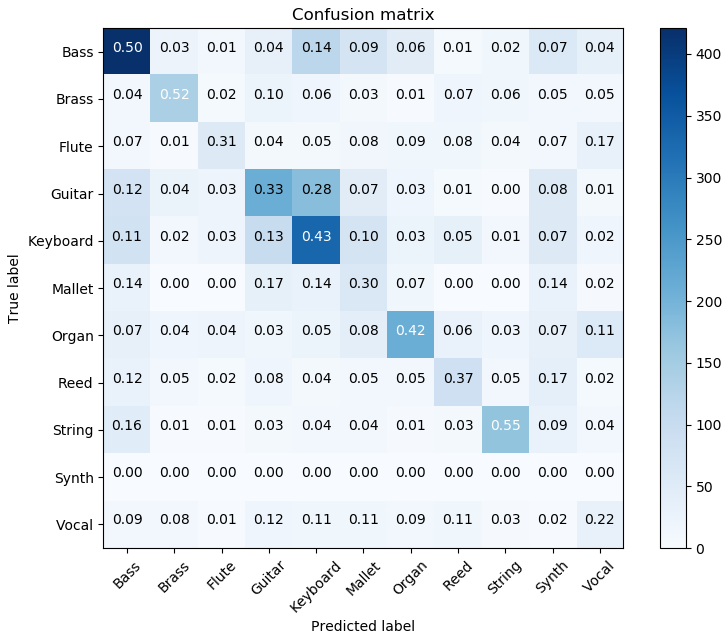
\includegraphics[width=0.8\textwidth]{confusion_top1.png}
\caption{Confusion matrix of results based on top one probability on testing sets}
\label{fig:confusionmatrix}
\end{figure}

% \begin{figure}[h!]
% \centering
% 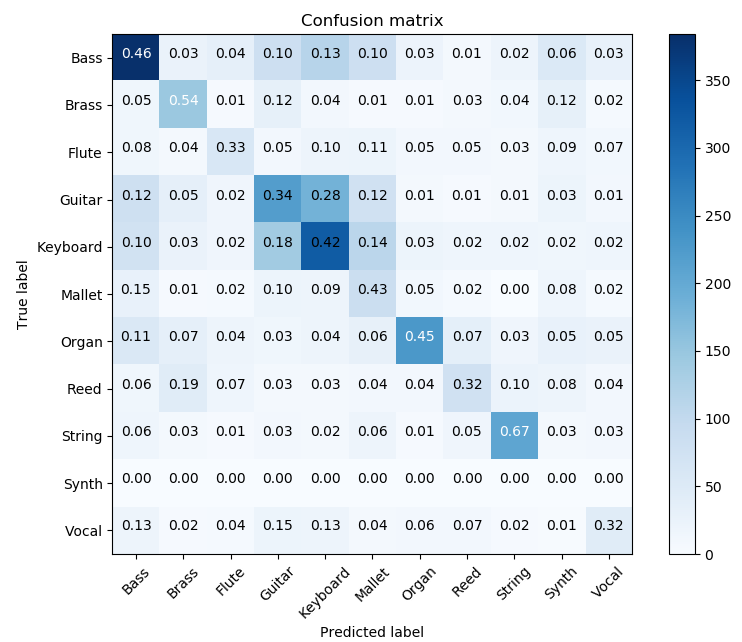
\includegraphics[width=0.8\textwidth]{confusion_top2.png}
% \caption{Confusion matrix of results based on top two probabilities on testing sets}
% \label{fig:confusionmatrix2}
% \end{figure}

% \noindent The instrument family name corresponds to their representing number is as in Table \ref{tab:confusionmatrix}.

% \begin{table}[h]
%   \caption{Instrument family names}
%   \label{tab:confusionmatrix}
%   \centering
%   \begin{tabular}{llllllllllll}
%     \toprule
%     Number  &0 &1 &2 &3 &4 &5\\
%     \midrule
%     Family name &Bass & Brass & Flute & Guitar & Keyboard &Mallet\\
%     \toprule
%     Number  &6 &7 &8 &9 &10\\
%     \midrule
%     Family name &Organ & Reed	& String    & Synth	& Vocal\\
%     \bottomrule
%   \end{tabular}
% \end{table}

\subsection{Play with real world music}

\noindent In order to test our model with real world music, we choose three different music files for testing. They are piano music from \emph{Days} playing by \emph{PianoBoy}, bass music from \emph{Pacific} playing by \emph{Rim Ramin Djawadi} and violin music from \emph{The Four Seasons (Spring)} playing by \emph{Joshua Bell}. After playing with the music, we got some practical results and did analysis based on it.

\begin{table}[h]
  \caption{Accuracy of three music based on top1 probability}
  \label{tab:3music_top1}
  \centering
  \begin{tabular}{lllllllllll}
    \toprule
    Music Name  &Bass & Brass & Flute & Guitar & Keyboard &Mallet\\
    &Organ & Reed	& String & Synth & Vocal\\
    \midrule
    Days (Piano) & 5.86\%& 10.03\%&6.02\%&9.57\%&\textbf{{\color{red} 12.50\%}}&2.31\%\\
    &2.78\%&\textbf{15.28\%}&\textbf{22.69\%}&5.56\%&7.41\%\\
    \midrule
    Pacific (Bass) & \textbf{{\color{red} 15.07\%}}&0.66\%&2.10\%&\textbf{14.95\%}&\textbf{14.40\%}&7.64\%\\
    &7.75\%&12.74\%&5.31\%&9.63\%&9.75\%\\
    \midrule
    Spring (Violin) & \textbf{10.11\%}&7.74\%&3.95\%&\textbf{12.32\%}&7.90\%&6.64\%\\
    &4.11\%&4.27\%&\textbf{{\color{red} 24.33\%}}&9.00\%&9.64\%\\
    \bottomrule
  \end{tabular}
\end{table}

\begin{table}[h]
  \caption{Accuracy of three music based on top2 probabilities}
  \label{tab:3music_top2}
  \centering
  \begin{tabular}{lllllllllll}
    \toprule
    Music Name  &Bass & Brass & Flute & Guitar & Keyboard &Mallet\\
    &Organ & Reed	& String & Synth & Vocal\\
    \midrule
    Days (Piano) & 7.25\%& 5.86\%&3.24\%&10.03\%&\textbf{{\color{red} 17.60\%}}&2.47\%\\
    &5.40\%&\textbf{14.97\%}&\textbf{24.07\%}&2.78\%&6.32\%\\
    \midrule
    Pacific (Bass) & \textbf{{\color{red} 16.17\%}}&1.77\%& 1.22\%&\textbf{11.96\%}&10.85\%&9.41\%\\
    &\textbf{17.39\%}&9.75\%&2.44\%&8.19\%&10.85\%\\
    \midrule
    Spring (Violin) & \textbf{13.27\%}&8.85\%&5.06\%&\textbf{12.16\%}&9.32\%&5.53\%\\
    &3.95\%&9.48\%&\textbf{{\color{red}19.43\%}}&5.85\%&7.11\%\\
    \bottomrule
  \end{tabular}
\end{table}

\noindent In order to recognize real world music, we need to consider the stride of the sliding window which is used to read the music and generate the predictions. The sampling rate of NSynth Dataset is 16,000 and each piece of available data has length of 3 seconds, which is 48,000 data in total. Thus, we use the same sample rate to read the record and the sliding window of our real music test is 3 seconds in order to generate one MFCCs feature since the data we used for training are all 3 seconds data. We then calculate the average time cost for computing one MFCCs features using our CNNs network. It is about 0.007 secs to generate one prediction in our network so that the stride should be no larger than this value. Thus we decided the stride of the window is 1 second which is easier to calculate.

\noindent The recognition results of the three pieces of music are as in Table \ref{tab:3music_top1} and Table \ref{tab:3music_top2}. We calculated the results of top one probability and top two probabilities for each sliding window of our real music. Then we counted the number of results of all sliding windows according to their classes and their portions among all the results as the recognition results. From the two tables, we can see that the results are relatively good. We know that \emph{Days} is piano music, which belongs to keyboard family. \emph{Pacific} is bass music, which belongs to bass family. And \emph{Spring} is violin music, which belongs to string family. The bold results are the three highest classes for each piece of music and the bold red results are their true classes. We can see that the three highest classes all contains the right class of the original music. The classes with the highest probabilities of \emph{Spring} in two tables are all corresponds to the right class. The right class of \emph{Pacific} is the highest probabilities in Table \ref{tab:3music_top1} and is the second highest in Table \ref{tab:3music_top2}, which is only a little less than the highest one. However, the right class of \emph{Days} are always the second highest while the highest is String. So, according to the results of real music, we conclude that in practice, our network sometimes confuses keyboard with string, but it can recognize string music and bass music with high probability.

% 我们可以看到每首音乐的识别结果(两个表),我们发现识别效果还是比较好的。我们选取最大的3个乐器里面都包含对应的乐器。比如dAYS里面keyboard,pacific里的bass,spring里面的strin。另外我们发现keyboard和string经常有混淆,在我们这个网络里面不容易分辨。小提琴音乐相对来说比较容易分辨,识别度比较高。

% \noindent When we test the model with pure piano music, it should always output "keyboard" prediction if it works well, however, it doesn't. When we use a sliding window with 4 second and feed the transformed mfcc data to the network, it gives us predictions randomly. We address the problem on the NSynth dataset. The last one second of our training data are mostly silent. So when we test with pure piano music, we change the size of sliding window to 3 seconds and add 1 second with zeros. In this time, "keyboard" always occurs in the top 3 prediction. But the network still gives "bass" prediction with high probability. We guess the problem is that the training data has too much low frequency component and the bass also has low frequency among all instruments. For mixture music, the network has bad performance (only produce random prediction).




\section{Discussion and Conclusions}

From the results of our experiments based on the parameter settings, we found that a relatively smaller batch size performs better. When batch size is bigger, more data will be given to the network to fit in each iteration. They can both converge to a relative small loss but large-batch methods tend to converge to sharp minimizers of the training and testing functions, and sharp minimizers lead to poorer generalization \cite{keskar}. Due to time limitation, we didn't try more batch sizes, but if time allows, it's better to try different batch sizes and choose the most suitable one.

% \noindent Moreover, we didn't expect that training the three subsets to perform better than training a whole training set together. But we think one reason behind it is that the training process performs much more iterations than training a whole training set with 20 epoches, as we can see from Figure \ref{fig:accuracy_loss_200} and Figure \ref{fig:accuracy_loss_200_apart} that the former only has 2000 iterations but the latter has 12000 iterations.

\noindent In the future, we plan to do some more experiments, such as trying more different parameter settings or tuning the networks to improve its performance. Also, we are now doing the single instrument recognition but we are also interested in mixture music instrument recognition. So we plan to add fusion data, which mixes different music instruments together randomly and has multiple labels, in order to give model ability of handling mixture music.

\noindent Finally, we conclude that CNNs are good models for music instruments recognition and the models also perform well in real life music. Also, we hope to discover more on this topic in the future.

% TODO:

% 1.DATA NORMALISZATION

% 2.conv filter

% 3.add one more fc layer

% \clearpage

\begin{thebibliography}{9}

\bibitem{sell}
Sell, Greg, Gautham J. Mysore, and Song Hui Chon. "Musical Instrument Detection." \textit{Center for Computer Research in Music and Acoustics} (2006).

\bibitem{deng}
Deng, Jeremiah D., Christian Simmermacher, and Stephen Cranefield. "A study on feature analysis for musical instrument classification." \textit{IEEE Transactions on Systems, Man, and Cybernetics, Part B (Cybernetics)} 38.2 (2008): 429-438.

\bibitem{agostini}
Agostini, Giulio, Maurizio Longari, and Emanuele Pollastri. "Musical instrument timbres classification with spectral features." \textit{EURASIP Journal on Advances in Signal Processing} 2003.1 (2003): 943279.

\bibitem{eronen}
Eronen, Antti. "Comparison of features for musical instrument recognition." \textit{Applications of Signal Processing to Audio and Acoustics, 2001 IEEE Workshop on the.} IEEE, 2001.

\bibitem{zhang}
Zhang, Wei, et al. "Computerized detection of clustered microcalcifications in digital mammograms using a shift‐invariant artificial neural network." \textit{Medical Physics} 21.4 (1994): 517-524.

\bibitem{krizhevsky}
Krizhevsky, Alex, Ilya Sutskever, and Geoffrey E. Hinton. "Imagenet classification with deep convolutional neural networks." \textit{Advances in neural information processing systems.} 2012.

\bibitem{vanden}
Van den Oord, Aaron, Sander Dieleman, and Benjamin Schrauwen. "Deep content-based music recommendation." \textit{Advances in neural information processing systems.} 2013.

\bibitem{abdelhamid}
Abdel-Hamid, Ossama, et al. "Convolutional neural networks for speech recognition." IEEE/ACM Transactions on audio, speech, and language processing 22.10 (2014): 1533-1545.

\bibitem{yoonchang}
Han, Yoonchang, et al. "Deep convolutional neural networks for predominant instrument recognition in polyphonic music." \textit{IEEE/ACM Transactions on Audio, Speech and Language Processing (TASLP)} 25.1 (2017): 208-221.

\bibitem{srivastava}
Srivastava, Nitish, et al. "Dropout: A simple way to prevent neural networks from overfitting." \textit{The Journal of Machine Learning Research} 15.1 (2014): 1929-1958.

\bibitem{adam}
Kingma, Diederik P., and Jimmy Ba. "Adam: A method for stochastic optimization." \textit{arXiv preprint arXiv:1412.6980} (2014).

\bibitem{nsynth}
Jesse Engel, Cinjon Resnick, Adam Roberts, Sander Dieleman, Douglas Eck,Karen Simonyan, and Mohammad Norouzi. "Neural Audio Synthesis of Musical Notes with WaveNet Autoencoders." 2017.

\bibitem{mfcc}
"Mel-Frequency Cepstrum." \texit{Wikipedia}, Wikimedia Foundation, 12 May 2018, en.wikipedia.org/wiki/Mel-frequency\_cepstrum.

\bibitem{keskar}
Keskar, Nitish Shirish, et al. "On large-batch training for deep learning: Generalization gap and sharp minima."\texit{ arXiv preprint arXiv:1609.04836} (2016).

\end{thebibliography}

\clearpage

\section*{Appendix -- Peer review}

\noindent \textbf{1. Relevance for the learning outcomes}

We agree with the advice of training network with multi-parameters. So we keep the model parameter as before and minimize the batch size properly to 200 after that the network finally has better performance than that with 400 batch size. We have shown the comparison result in report. But in order to have a more accurate gradient descent, we did not try too small batch size. 

Because of the time limitation, we did not do many experiment with different parameter.

\noindent \textbf{2. Literature study}

Firstly, we think there's no need to add performance of other models using different datasets because different datasets will result in very different results. So we don't think comparing them with our model is a good idea.

Then, we've add more descriptions about that CNNs are shift invariant, so that it would be more logical.

We also add the recommended paper about applying CNN to music samples because we think this is indeed what was missing before.

About the two assumptions in model architecture, we write the two assumptions according to our own understanding of CNNs. For the first one, we know convolutional kernels are to extract part of the image so bigger size means bigger part, thus means more detailed image. As for the second one, it is the visual explanation of the pooling layer. We think these two assumptions are relevant to what we explained together with them, so it's our own understanding and there's no need to find a paper and cite them from the paper.

\noindent \textbf{3. Novelty/Originality}

There's no suggestions so nothing to explain here.

\noindent \textbf{4. Correctness}

Here are explanations of each comment.

3.1 Data-preprocessing: In order to do data balance, we randomly choose 10,000 samples from each class with replacement, which has been clarified in the report now. So the whole training dataset has 110,000 samples and each class has the same number of samples.

4. Result: The figures with accuracy and loss have been smoothed so that we can easier see the trend of accuracy and loss. We can see that in these two figures, the results of validation(blue line) vary a lot that is because we randomly chose 200 samples from validation set each time to calculate the accuracy and loss. It is normal that we got the similar result in testing set and validation set which means our network works well. We replicated the experiment and found the result are quite similar so we just show one pair of result in our report. As for the gap mentioned in peer review, we don't understand it very much, but we've clarified our loss and accuracy curve figure so we think it can now help you understand.

%Did you notice any important difference between the these testing/validation set and the training that could explain this gap otherwise ?

4.4 Confusion matrix: We have the new confusion matrix after normalization in our report with label and value which is easier understanding. And we only use the whole testing set to calculate the confusion matrix now rather randomly selecting samples according to the advice. 

\noindent \textbf{5. Clarity of presentation}

1. Introduction: According to the advice, we modified our goal more precise and add the point that we apply our network on real music.

%2.1 两个model architecture
2.1 Model architecture(1): According to the advice, we added the amount of parameters for CNNs in our paper. We used our own calculation instead of the calculation from the peer review.

2.1 Model architecture(2): We changed explanations about the pooling layer so that it's more clear. We also added the detailed value of the settings and include the recommended paper.

2.2.2 Feature extraction: According to the advice, when we enframe the samples, we also need to consider the value of frame length in samples and the shift of consecutive windows in samples. Now this has already been clarified in our paper.

3.2 Experimental setup: It is true that we finally only has 2 coefficient output after the convolutional network for the second dimension before going into fully connection layer. We think that is the reason why the performance cannot be improved very well since we lose some information in this dimension. We agree that reducing the kernel size, adding padding or change the kernel size to rectangle instead of square can better preserve information, which can be our future work.

4. Results: First we only calculated the accuracy based on the top probability prediction. According to the advice, we added an evaluation method that calculates the accuracy based on top two probabilities in prediction. We made comparison of these two evaluation methods. The accuracy in validation set and testing set has great improvements. The results of confusion matrix of these two evaluation methods are quite similar, which means those classes with higher classification accuracy are same, so we only show the result of one in the report.

4.4 Confusion matrix: We've add the colormap and class names and generate a more clear figure of confusion matrix.

4.5 Play with real world music: In the draft, we only describe this part generally because we hadn't finished that part of experiments at that time. The sliding window is to recognize the music because the music is very long while our training data only have 3 seconds. Now the part has been more clarified. The advice of using smaller windows is good but we didn't have time to experiment.


% \noindent \textbf{Conclusion}

% The advice are quite helpful and we modified the report according to these. Testing on real data is quite difficult and challenging but interesting.  

\end{document}